%%%%%%%%%%%%%%%%%%%%%%%%%%%%%%%%%%%%%%%%%%%%%%%%%%%%%%%%%%%%%%%%%%%%%%
% Lớp 10 | Véctơ (chưa xét tọa độ) | Tích vô hướng (chưa xét tọa độ)
% Dạng 0H5?4-7: Toán thực tế  áp dụng tích vô hướng
%%%%%%%%%%%%%%%%%%%%%%%%%%%%%%%%%%%%%%%%%%%%%%%%%%%%%%%%%%%%%%%%%%%%%%


% nguồn: gemini-code-1794580744144 (nhập 13/11/2026)
\begin{ex}%[0H5V4-7]%[ma:623b92a7]
	Một chiếc xe được kéo bởi một lực $\overrightarrow{F}$ có độ lớn $50 \text{ N}$, di chuyển theo một đường thẳng từ $A$ đến $B$ với chiều dài $150 \text{ m}$. Cho biết góc hợp bởi lực kéo $\overrightarrow{F}$ và hướng dịch chuyển $\overrightarrow{AB}$ bằng $30^\circ$. Kí hiệu công sinh ra bởi lực $\overrightarrow{F}$ là $A = \overrightarrow{F} \cdot \overrightarrow{AB}$. Các mệnh đề sau đúng hay sai?
	\choiceTF
	{\True Độ lớn của vectơ dịch chuyển $\overrightarrow{AB}$ là $|\overrightarrow{AB}| = 150 \text{ m}$}
	{\True Độ lớn của lực kéo là $|\overrightarrow{F}| = 50 \text{ N}$}
	{Công sinh ra bởi lực kéo $\overrightarrow{F}$ được tính bằng công thức $A = |\overrightarrow{F}| \cdot |\overrightarrow{AB}| \cdot \sin 30^\circ$}
	{\True Công sinh ra bởi lực kéo $\overrightarrow{F}$ là $3750\sqrt{3} \text{ (J)}$}
	\loigiai{
		\begin{itemchoice}
			\itemch Đúng. Quãng đường vật di chuyển từ $A$ đến $B$ dài $150 \text{ m}$ nên $|\overrightarrow{AB}| = 150$.
			\itemch Đúng. Theo giả thiết, độ lớn của lực kéo $\overrightarrow{F}$ là $50 \text{ N}$.
			\itemch Sai. Theo định nghĩa tích vô hướng, công sinh ra được tính bằng $A = \overrightarrow{F} \cdot \overrightarrow{AB} = |\overrightarrow{F}| \cdot |\overrightarrow{AB}| \cdot \cos(\overrightarrow{F}, \overrightarrow{AB}) = |\overrightarrow{F}| \cdot |\overrightarrow{AB}| \cdot \cos 30^\circ$.
			\itemch Đúng. Thay số vào công thức ta được $A = 50 \cdot 150 \cdot \cos 30^\circ = 7500 \cdot \dfrac{\sqrt{3}}{2} = 3750\sqrt{3} \text{ (J)}$.
		\end{itemchoice}
	}
\end{ex}

% nguồn: gemini-code-1794581230180 (nhập 13/11/2026)
\begin{ex}%[0H5V4-7] % KIEM_TRA: Toán thực tế áp dụng tích vô hướng và công của lực%[ma:9fcb1226]
	Một chiếc xe được kéo bởi một lực $\overrightarrow{F}$ có độ lớn $50\text{ N}$, di chuyển theo một đường thẳng từ $A$ đến $B$ với chiều dài $150\text{ m}$. Góc hợp bởi lực kéo $\overrightarrow{F}$ và hướng dịch chuyển $\overrightarrow{AB}$ bằng $30^\circ$. Lực $\overrightarrow{F}$ được phân tích thành hai lực thành phần vuông góc là $\overrightarrow{F_1}$ và $\overrightarrow{F_2}$, trong đó $\overrightarrow{F_1}$ cùng hướng với $\overrightarrow{AB}$. Các mệnh đề sau đúng hay sai?
	\choiceTF
	{\True Độ lớn của vectơ dịch chuyển $\overrightarrow{AB}$ là $|\overrightarrow{AB}| = 150$}
	{Công sinh ra bởi lực kéo $\overrightarrow{F}$ được tính bằng công thức $A = |\overrightarrow{F}| \cdot |\overrightarrow{AB}| \cdot \sin 30^\circ$}
	{\True Công sinh ra bởi lực $\overrightarrow{F}$ là $3750\sqrt{3}\text{ (J)}$}
	{Lực $\overrightarrow{F_2}$ sinh công lớn hơn $0$}
	\loigiai{
		\begin{itemchoice}
			\itemch Đúng. Quãng đường vật di chuyển từ $A$ đến $B$ dài $150\text{ m}$ nên $|\overrightarrow{AB}| = 150$.
			\itemch Sai. Công sinh ra bởi lực kéo $\overrightarrow{F}$ được tính bằng tích vô hướng: $A = \overrightarrow{F} \cdot \overrightarrow{AB} = |\overrightarrow{F}| \cdot |\overrightarrow{AB}| \cdot \cos 30^\circ$.
			\itemch Đúng. Thay số vào công thức ta được: \\
			\[ A = 50 \cdot 150 \cdot \cos 30^\circ = 7500 \cdot \frac{\sqrt{3}}{2} = 3750\sqrt{3}\text{ (J)} \]
			\itemch Sai. Vì lực $\overrightarrow{F_2}$ vuông góc với hướng dịch chuyển $\overrightarrow{AB}$ nên $\overrightarrow{F_2} \cdot \overrightarrow{AB} = 0$, suy ra lực $\overrightarrow{F_2}$ không sinh công (công bằng $0$).
		\end{itemchoice}
	}
\end{ex}

% nguồn: TuLuan_Lop10_Dot2 (nhập 14/11/2026)
% nguồn: TuLuan_Lop10_Dot2 (nhập 14/11/2026)
\begin{bt}%[0H5H4-7]%[Dự án đề kiểm tra HKII NH22-23 - Thy Nguyen Vo Diem]%[THPT Trần Quang Khải]%[ma:ffd99988]
Một người dùng một lực $\overrightarrow{F}$ có độ lớn $100 $N để kéo một thùng hàng dịch chuyển một đoạn $15$m. Biết lực $\overrightarrow{F}$ hợp với hướng dịch chuyển một góc $60^{\circ}$. Tính công sinh bởi lực $\overrightarrow{F}$.
\loigiai{
\immini{Công sinh bởi lực $\overrightarrow{F}$ là $$\left|\overrightarrow{F}\right| \left|\overrightarrow{d} \right|\cos \left(\overrightarrow{F},\overrightarrow{d}\right)=100 \cdot 15 \cdot \cos 60^\circ=750 \ (\mathrm{N}).$$}{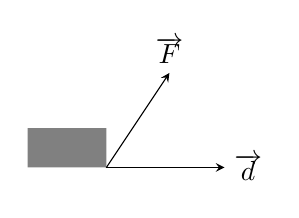
\begin{tikzpicture}[>=stealth,scale=1, line join = round, line cap = round]
	\fill[gray] (0,0)--(0,0.5)--(1,0.5)--(1,0)--(0,0);
	\draw[->] (1,0)--(2.5,0) node[right]{$\overrightarrow{d}$};
	 \draw[->] (1,0)--(1.8,1.2) node[above]{$\overrightarrow{F}$};
\end{tikzpicture}
}
}
\end{bt}

% nguồn: TuLuan_Lop10_Dot2 (nhập 14/11/2026)
\begin{bt}%[0H5H4-7]%[Dự án đề kiểm tra HKI NH22-23 - Quan Ón]%[Giồng Ông Tố]%[ma:8095850f]
	Tính công sinh bởi một lực $\overrightarrow{F}$ có độ lớn $60$ N kéo một vật dịch chuyển một véc-tơ $\overrightarrow{d}$ có độ dài $200$ m. Cho biết $\left( \overrightarrow{F}, \overrightarrow{d} \right) = 60^\circ$.
	\dapso{$6000$ J.}
	\loigiai{
		Công sinh bởi lực $\overrightarrow{F}$ là
		$$ \overrightarrow{F}\cdot \overrightarrow{d} = \left|\overrightarrow{F} \right|\cdot \left|\overrightarrow{d} \right|\cdot \cos 60^\circ = 60\cdot 200\cdot \dfrac{1}{2} = 6000 \quad \textrm{(J).}$$
	}
\end{bt}

% nguồn: TuLuan_Lop10_Dot2 (nhập 14/11/2026)
% nguồn: TuLuan_Lop10_Dot2 (nhập 14/11/2026)
% nguồn: TuLuan_Lop10_Dot2 (nhập 14/11/2026)
\begin{bt}%[0H5H4-7]%[Dự án đề kiểm tra HKI NH22-23-Trương Đăng Khoa]%[THPT Nguyễn Công Trứ]%[ma:57139a83]
	Một vật trượt trên sàn dưới tác dụng của một lực không đổi $\overrightarrow{F}$ có độ lớn $20$ N, hợp với hướng chuyển động của vật một góc $30^\circ$. Tính công $A$ sinh ra bởi lực $\overrightarrow{F}$ biết vật di chuyển được một quãng đường bằng $20\,\mathrm{m}$.
	\loigiai{Công $A$ sinh ra là $A=F\cdot s\cdot \cos 3\alpha =20\cdot 20\cdot \cos 30=200\sqrt{3}$ $\mathrm{J}$.}
\end{bt}

% nguồn: TuLuan_Lop10_Dot2 (nhập 14/11/2026)
\begin{bt}%[0H5V4-7]%[ma:b6b1043e]
	Cho ba điểm $M$, $N$, $P$. Nếu một lực $\overrightarrow{F}$ không đổi tác động lên một chất điểm trong suốt quá trình chuyển động của chất điểm, thì các công sinh bởi lực $\overrightarrow{F}$ trong hai trường hợp sau có mối quan hệ gì với nhau?
	\begin{enumerate}
		\item Chất điểm chuyển động theo đường gấp khúc từ $M$ đến $N$ rồi tiếp tục từ $N$ đến $P$.
		\item Chất điểm chuyển động thằng từ $M$ đến $P$.
	\end{enumerate}
	\loigiai
	{
		Do lực $\overrightarrow{F}$ không đổi, tác động lên chất điểm trong suốt quá trình chuyển động của chất điểm, nên công sinh bởi lực $\overrightarrow{F}$ khi chất điểm chuyển động theo đường gấp khúc từ $M$ tới $N$ rồi từ $N$ tới $P$ bằng $A_{1}=\overrightarrow{F} \cdot \overrightarrow{M N}+\overrightarrow{F} \cdot \overrightarrow{N P}$ (1) và công sinh bởi lực $F$ khi chất điểm chuyển động thẳng từ $M$ tới $P$ bằng
		\[A_2=\overrightarrow{F}\cdot\overrightarrow{MP}\quad(2)\]
		Từ $(1)$ và $(2)$ để ý rằng $\overrightarrow{MP}=\overrightarrow{MN}+\overrightarrow{NP}$ suy ra $A_1=A2$.
	}
\end{bt}

% nguồn: TuLuan_Lop10_Dot2 (nhập 14/11/2026)
\begin{bt}%[0H5H4-7]%[ma:6ad61c6b]
	Tính công sinh bởi một lực $\overrightarrow{F}$ có độ lớn $20$ N kéo một vật dịch chuyển theo một véc-tơ $\overrightarrow{d}$ có độ dài $50$ m và cho biết $(\overrightarrow{F},\overrightarrow{d})=60^\circ$.
	\loigiai{
		Ta có $A=\overrightarrow{F}\cdot \overrightarrow{d}=|\overrightarrow{F}|\cdot |\overrightarrow{d}|\cdot \cos(\overrightarrow{F},\overrightarrow{d})=20\cdot 50\cdot \cos 60^\circ=20\cdot 50\cdot \dfrac{1}{2}=500$ J.
	}
\end{bt}

% nguồn: TuLuan_Lop10_Dot2 (nhập 14/11/2026)
\begin{bt}%[0H5H4-7]%[Tex hóa SGK CD-CT,T7/22, Trần Nhân Kiệt]%[ma:0a79778e]
	Tính công sinh bởi một lực $\overrightarrow{F}$ có độ lớn $60$ N kéo một vật di chuyển một véc-tơ $\overrightarrow{d}$ có độ dài $200$ m. Cho biết $(\overrightarrow{F},\overrightarrow{d})=60^\circ$.
	\loigiai{
		Ta có $A=\overrightarrow{F}\cdot \overrightarrow{d}=|\overrightarrow{F}|\cdot |\overrightarrow{d}|\cdot \cos(\overrightarrow{F},\overrightarrow{d})=60\cdot 200\cdot \cos 60^\circ=60\cdot 200\cdot \dfrac{1}{2}=6000$ J.
	}
\end{bt}

% nguồn: TuLuan_Lop10_Dot2 (nhập 14/11/2026)
\begin{bt}%[0H5V4-7]%[ma:8377bd22]
	Một ô tô có khối lượng $2{,}5$ tấn chạy từ chân lên đỉnh một con dốc thẳng.	Tính công của trọng lực tác động lên xe, biết dốc dài $50 \mathrm{m}$ và nghiêng $15^{\circ}$ so với phương nằm ngang (trong tính toán, lấy gia tốc trọng trường bằng $10 \mathrm{~m} / \mathrm{s}^{2}$)
	\loigiai{
	\begin{center}
		\begin{tikzpicture}[scale=1, font=\footnotesize, line join=round, line cap=round, >=stealth]
			\path (0,0) coordinate (A) ++(180:8) coordinate (B) ++(15:8.28) coordinate (C) (-3,2) coordinate (M) (-3,0.5) coordinate (P) node[left]{$\overrightarrow{P}$}(-1.01,2.53) coordinate (N) node[above]{$N$} (-2.63,0.6) coordinate (E) node[right]{$\overrightarrow{P}_1$} (-3.38,1.9) coordinate (F) node[left]{$\overrightarrow{P}_2$};
			\draw[dashed] (A)--(B) (E)--(P)--(F);
			\draw (B)--(C);
			\draw[-stealth] (M)--(P);\draw [-stealth](M)--(E);\draw [-stealth](M)--(F); \draw[-stealth,dashed] (M)--(N);
			\draw pic["$15^\circ$" shift={(1cm,1mm)},draw, double, angle radius =1.5cm]{angle=A--B--C};
			\draw pic["$105^\circ$" shift={(0.5cm,-0.1cm)},draw, angle radius =0.3cm]{angle=P--M--N};
			\fill (M) circle (1.5pt) node[above]{$M$};
		\end{tikzpicture}
	\end{center}
	Trọng lực của ô tô có độ lớn bằng $|\overrightarrow{P}|=2500 \times 10=25000(\mathrm{~N})$.\\
	Trọng lực $\overrightarrow{P}$ của ô tô hợp với hướng chuyển dời $\overrightarrow{M N}$ một góc $\alpha=90^{\circ}+15^{\circ}=105^{\circ}$.\\
	Trọng lực $\overrightarrow{P}$ được phân tích thành hai thành phần $\overrightarrow{P_{1}}$ và $\overrightarrow{P_{2}}: \overrightarrow{P}=\overrightarrow{P_{1}}+\overrightarrow{P_{2}}$,
	trong đó $\overrightarrow{P_{1}}$ có phương vuông góc với mặt dốc, $\overrightarrow{P_{2}}$ có phương song song với mặt dốc.\\
	Ta nhận thấy rằng, $\overrightarrow{P_{1}}$ không có tác dụng đối với chuyển dời $\overrightarrow{M N}$ của xe, còn $\overrightarrow{P_{2}}$ ngược hướng với $\overrightarrow{MN}$.\\
	Do đó, công của trọng lực tác động lên xe bằng
	$$
	\begin{aligned}
		A &=\overrightarrow{P} \cdot \overrightarrow{M N}=|\overrightarrow{P}| \cdot|\overrightarrow{M N}| \cdot \cos (\overrightarrow{P} ; \overrightarrow{M N}) \\
		&=25000 \cdot 50 \cdot \cos 105^{\circ} \approx-323524(\mathrm{~J}) .
	\end{aligned}
	$$
	\textbf{Nhận xét.} Cũng có thể tính công $A$ nhờ định lí chiếu (xem mục Nhận xét sau Ví dụ 2, Bài 11) như sau:
	$$
	\begin{aligned}
		A &=\overrightarrow{P} \cdot \overrightarrow{M N}=\overrightarrow{P_{2}} \cdot \overrightarrow{M N}=\left|\overrightarrow{P_{2}}\right| \cdot|\overrightarrow{M N}| \cdot \cos 180^{\circ} \\
		&=-\left(|\overrightarrow{P}| \cdot \sin 15^{\circ}\right) \cdot 50 \approx-323524(\mathrm{~J}) .
	\end{aligned}
	$$
	}
\end{bt}

% nguồn: ThucTe_Lop10_TLN_DS (nhập 14/11/2026)
\begin{bt}%[0H5H4-7]%[ma:a85b45a6]
Một người dùng một lực $\overrightarrow{F}$ có độ lớn là $90$ N làm một vật dịch chuyển một đoạn $100$ m. Biết lực hợp $\overrightarrow{F}$ hợp với hướng dịch chuyển một góc $60^{\circ}$. Tính công sinh bởi lực $\overrightarrow{F}$. 
\shortans{$4500$}
\loigiai{
\immini
{
	Công sinh bởi lực $\overrightarrow{F}$ được tính bằng công thức\\
	$\overrightarrow{F}\cdot \overrightarrow{d}=\left|\overrightarrow{F}\right|\cdot \left|\overrightarrow{d}\right|\cdot \cos \left(\overrightarrow{F},\overrightarrow{d}\right)=90\cdot 100\cdot \cos 60^{\circ}=4500$ (J).
}{
		\begin{tikzpicture}[scale=1,font=\footnotesize, line join=round, line cap=round, >=stealth]
		\path
		(0,0) coordinate (A)		
		(4,0) coordinate (B)		
		(1,2) coordinate (C)		
		;
		\draw[->] (A)--(B);
		\draw[->] (A)--(C);
		\pic[draw,"$60^{\circ}$", angle eccentricity=.7,angle radius=0.7cm]{angle=B--A--C};
		\path (A)--(C) node[left,midway]{$\overrightarrow{F}$};
		\path (A)--(B) node[above,midway]{$\overrightarrow{d}$};
		\path (A)--(C) node[right,midway]{$90$ N};
		\path (A)--(B) node[below,midway,sloped]{$100$ m};
		\foreach \x/\g in {A/90,B/0,C/-90} \fill[black] (\x) circle (1pt);
	\end{tikzpicture}
}


}
\end{bt}

% nguồn: De_AI_Toan10_cuoi_hoc_ki_i_1 (nhập 21/11/2026)
\begin{ex}%[0H5H4-7]%[ma:40efa713]
	Một người kéo một thùng hàng trên mặt phẳng nằm ngang bằng một lực $\overrightarrow{F}$ không đổi có độ lớn $80\text{ N}$, hợp với phương ngang (hướng chuyển động) một góc $60^\circ$. Thùng hàng dịch chuyển thẳng một quãng đường $10\text{ m}$ từ $A$ đến $B$. Biết công cơ học sinh bởi một lực không đổi $\overrightarrow{F}$ trên độ dịch chuyển $\overrightarrow{AB}$ là $A=\overrightarrow{F}\cdot\overrightarrow{AB}$. Xét tính đúng, sai của các khẳng định sau:
	\choiceTF
	{\True Độ dài của vectơ độ dịch chuyển $\overrightarrow{AB}$ là $10\text{ m}$.}
	{Công sinh bởi lực kéo $\overrightarrow{F}$ trên quãng đường $AB$ bằng $400\sqrt{3}\text{ J}$.}
	{\True Trọng lực $\overrightarrow{P}$ tác dụng lên thùng hàng (có phương thẳng đứng, hướng xuống dưới) sinh công bằng $0\text{ J}$.}
	{\True Nếu có thêm lực ma sát $\overrightarrow{F}_{ms}$ ngược hướng chuyển động với độ lớn $25\text{ N}$ thì tổng công của lực kéo $\overrightarrow{F}$ và lực ma sát $\overrightarrow{F}_{ms}$ trên quãng đường $AB$ bằng $150\text{ J}$.}
	\loigiai{
		\begin{itemchoice}
			\itemch Đúng. Thùng hàng dịch chuyển thẳng $10\text{ m}$ từ $A$ đến $B$ nên $|\overrightarrow{AB}|=10\text{ m}$.
			\itemch Sai. Công của lực kéo là $A=\overrightarrow{F}\cdot\overrightarrow{AB}=80\cdot 10\cdot\cos 60^\circ=800\cdot 0{,}5=400\text{ J}$.
			\itemch Đúng. Vì trọng lực $\overrightarrow{P}$ vuông góc với vectơ độ dịch chuyển $\overrightarrow{AB}$ nên $A_P=\overrightarrow{P}\cdot\overrightarrow{AB}=0\text{ J}$.
			\itemch Đúng. Công của lực ma sát là $A_{ms}=25\cdot 10\cdot\cos 180^\circ=-250\text{ J}$, suy ra tổng công bằng $400+(-250)=150\text{ J}$.
		\end{itemchoice}
	}
\end{ex}

% nguồn: De_AI_Toan10_cuoi_hoc_ki_i_1 (nhập 21/11/2026)
\begin{ex}%[0H5H4-7]%[ma:4680b562]
	Một chiếc thuyền chuyển động thẳng từ bến $A$ đến bến $B$ với vectơ độ dịch chuyển $\overrightarrow{d}=\overrightarrow{AB}$ có độ dài $50\text{ m}$. Thuyền đồng thời chịu tác dụng của lực đẩy động cơ $\overrightarrow{F}_1$ (cùng hướng với $\overrightarrow{d}$, độ lớn $200\text{ N}$) và lực gió $\overrightarrow{F}_2$ (có độ lớn $100\text{ N}$, hợp với hướng chuyển động $\overrightarrow{d}$ một góc $120^\circ$). Xét tính đúng, sai của các khẳng định sau:
	\choiceTF
	{\True Công của lực đẩy động cơ $\overrightarrow{F}_1$ sinh ra trên đoạn đường $AB$ là $10000\text{ J}$.}
	{Công của lực gió $\overrightarrow{F}_2$ sinh ra trên đoạn đường $AB$ là $2500\text{ J}$.}
	{\True Độ lớn của hợp lực $\overrightarrow{F}=\overrightarrow{F}_1+\overrightarrow{F}_2$ bằng $100\sqrt{3}\text{ N}$.}
	{\True Góc tạo bởi hợp lực $\overrightarrow{F}$ và vectơ độ dịch chuyển $\overrightarrow{d}$ bằng $30^\circ$.}
	\loigiai{
		\begin{itemchoice}
			\itemch Đúng. Ta có $A_1=\overrightarrow{F}_1\cdot\overrightarrow{d}=200\cdot 50\cdot\cos 0^\circ=10000\text{ J}$.
			\itemch Sai. Ta có $A_2=\overrightarrow{F}_2\cdot\overrightarrow{d}=100\cdot 50\cdot\cos 120^\circ=5000\cdot(-0{,}5)=-2500\text{ J}$.
			\itemch Đúng. Ta có $|\overrightarrow{F}|^2=|\overrightarrow{F}_1|^2+|\overrightarrow{F}_2|^2+2\overrightarrow{F}_1\cdot\overrightarrow{F}_2=200^2+100^2+2\cdot 200\cdot 100\cdot\cos 120^\circ=30000\Rightarrow|\overrightarrow{F}|=100\sqrt{3}\text{ N}$.
			\itemch Đúng. Ta có $\overrightarrow{F}\cdot\overrightarrow{d}=(\overrightarrow{F}_1+\overrightarrow{F}_2)\cdot\overrightarrow{d}=A_1+A_2=7500$, suy ra $\cos(\overrightarrow{F},\overrightarrow{d})=\dfrac{7500}{100\sqrt{3}\cdot 50}=\dfrac{\sqrt{3}}{2}\Rightarrow(\overrightarrow{F},\overrightarrow{d})=30^\circ$.
		\end{itemchoice}
	}
\end{ex}
